\documentclass[tikz,border=3pt]{standalone}
\usepackage[utf8]{inputenc}
\usepackage{xcolor}
\usepackage{tikz}

\begin{document}
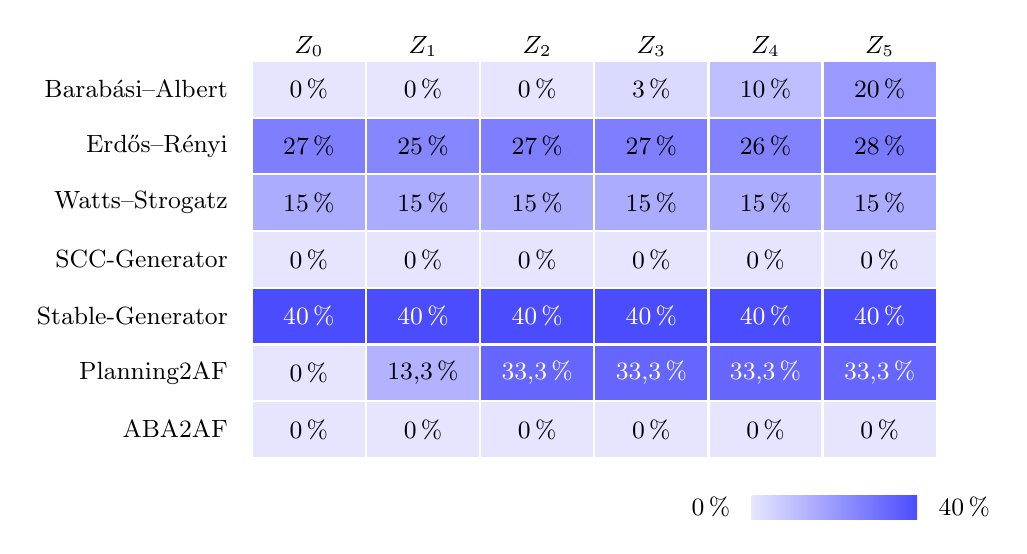
\begin{tikzpicture}[font=\small]
    \def\cellw{1.45}
    \def\cellh{0.72}

    \foreach [count=\col from 0] \label in {0,1,2,3,4,5} {
        \node at ({\col*\cellw+0.5*\cellw},{7*\cellh+0.18}) {$Z_{\label}$};
    }

    \newcommand{\drawfamilyrow}[3]{%
        \node[anchor=east] at (-0.18,{#1*\cellh+0.5*\cellh}) {#2};
        \foreach [count=\col from 0] \value in {#3} {
            \pgfmathsetmacro{\mix}{10+1.5*\value}
            \pgfmathtruncatemacro{\dark}{\value>28}
            \ifnum\dark=1\def\textcolor{white}\else\def\textcolor{black}\fi
            \fill[blue!\mix!white]
                ({\col*\cellw},{#1*\cellh})
                rectangle ++(\cellw,\cellh);
            \draw[white,line width=0.8pt]
                ({\col*\cellw},{#1*\cellh})
                rectangle ++(\cellw,\cellh);
            \node[text=\textcolor]
                at ({\col*\cellw+0.5*\cellw},{#1*\cellh+0.5*\cellh})
                {\pgfmathprintnumber[
                    fixed,precision=1,use comma
                ]{\value}\,\%};
        }
    }
    \drawfamilyrow{0}{ABA2AF}{0,0,0,0,0,0}
    \drawfamilyrow{1}{Planning2AF}{0,13.333,33.333,33.333,33.333,33.333}
    \drawfamilyrow{2}{Stable-Generator}{40,40,40,40,40,40}
    \drawfamilyrow{3}{SCC-Generator}{0,0,0,0,0,0}
    \drawfamilyrow{4}{Watts--Strogatz}{15,15,15,15,15,15}
    \drawfamilyrow{5}{Erdős--Rényi}{27,25,27,27,26,28}
    \drawfamilyrow{6}{Barabási--Albert}{0,0,0,3,10,20}

    \node[anchor=east] at ({6*\cellw-2.5},{-0.62}) {0\,\%};
    \shade[left color=blue!10!white,right color=blue!70!white]
        ({6*\cellw-2.35},{-0.78}) rectangle ({6*\cellw-0.25},{-0.48});
    \node[anchor=west] at ({6*\cellw-0.10},{-0.62}) {40\,\%};
\end{tikzpicture}
\end{document}
